\documentclass[../main.tex]{subfile}

\begin{document}

\tikzset{/tkzmkangle/mark=none}

\topictitle{Common Graphs}

In this section, $a, p, q \in \mathbb{R}$, $b \in \mathbb{N}$.

\figureWithThreeThings{
	\labeledDiagram{$r = a$}{
	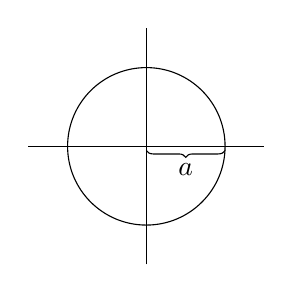
\begin{tikzpicture}
		\draw (-1.5,0) -- (1.5,0);
		\draw (0,-1.5) -- (0,1.5);
		\clip (1.5,1.5) rectangle (-1.5,-1.5);
		\coordinate (O) at (0,0);

		\draw (O) circle[radius=1];
		\draw[decorate, decoration={brace, amplitude=2.5pt, raise=1.5pt, mirror}]
			(O) -- node[below, yshift=-1mm] {$a$} (1,0);
	\end{tikzpicture}
}}{
	\labeledDiagram{$\theta = \alpha$}{
	\begin{tikzpicture}
		\draw (-0.5,0) -- (1.5,0);
		\draw (0,-0.5) -- (0,1.5);
		\clip (1.5,1.5) rectangle (-0.5,-0.5);
		\coordinate (O) at (0,0);

		\coordinate (A) at (2,3);
		\coordinate (B) at (1,0);
		\draw (O) -- (A);
		\tkzMarkAngle[size=0.8](B,O,A);
		\tkzLabelAngle[pos=0.52](B,O,A){$\alpha$};
	\end{tikzpicture}
}}{
	\labeledDiagram{$r = a\theta$}{
	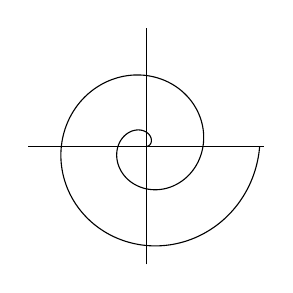
\begin{tikzpicture}
		\draw (-1.5,0) -- (1.5,0);
		\draw (0,-1.5) -- (0,1.5);
		\clip (1.5,1.5) rectangle (-1.5,-1.5);
		\coordinate (O) at (0,0);

		\draw [domain=0:720, smooth, samples=500] plot (\x:{0.002*\x});
	\end{tikzpicture}
}}

\figureWithThreeThings{
	\labeledDiagram{$r = a(p + q\cos\theta)\ (p = q)$}{
	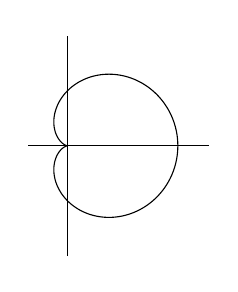
\begin{tikzpicture}
		\draw (-0.5,0) -- (1.8,0);
		\draw (0,-1.4) -- (0,1.4);
		\clip (1.5,1.5) rectangle (-0.5,-1.5);
		\coordinate (O) at (0,0);

		\draw[domain=0:360, smooth, samples=500] plot (\x:{0.7 * (1 + cos(\x))});
	\end{tikzpicture}
}}{
	\labeledDiagram{$r = a(p + q\cos\theta)\ (p \ge 2q)$}{
	\begin{tikzpicture}
		\draw (-0.65,0) -- (1.8,0);
		\draw (0,-1.4) -- (0,1.4);
		\clip (1.5,1.5) rectangle (-0.5,-1.5);
		\coordinate (O) at (0,0);

		\draw[domain=0:360, smooth, samples=500] plot (\x:{0.4 * (2 + cos(\x))});
	\end{tikzpicture}
}}{
	\labeledDiagram{$r = a(1 + \cos\theta)\ (q \le p < 2q)$}{
	\begin{tikzpicture}
		\draw (-0.55,0) -- (1.8,0);
		\draw (0,-1.4) -- (0,1.4);
		\clip (1.5,1.5) rectangle (-0.5,-1.5);
		\coordinate (O) at (0,0);

		\draw[domain=0:360, smooth, samples=500] plot (\x:{0.55 * (1.25 + cos(\x))});
	\end{tikzpicture}
}}

\figureWithThreeThings{
	\labeledDiagram{$r = a\sin b \theta\ (b = 3)$}{
	
\begin{tikzpicture}
		\draw (-1.5,0) -- (1.5,0);
		\draw (0,-1.5) -- (0,1.5);
		\clip (1.5,1.5) rectangle (-1.5,-1.5);
		\coordinate (O) at (0,0);

		\draw[domain=0:360, smooth, samples=500] plot (\x:{1.3 * sin(3 * \x)});
	\end{tikzpicture}
}}{
	\labeledDiagram{$r = a\cos b \theta\ (b = 3)$}{
	
\begin{tikzpicture}
		\draw (-1.5,0) -- (1.5,0);
		\draw (0,-1.5) -- (0,1.5);
		\clip (1.5,1.5) rectangle (-1.5,-1.5);
		\coordinate (O) at (0,0);

		\draw[domain=0:360, smooth, samples=500] plot (\x:{1.3 * cos(3 * \x)});
	\end{tikzpicture}
}}{
	\labeledDiagram{$r^2 = a^2\cos b \theta\ (b = 3)$}{
	
\begin{tikzpicture}
		\draw (-1.5,0) -- (1.5,0);
		\draw (0,-1.5) -- (0,1.5);
		\clip (1.5,1.5) rectangle (-1.5,-1.5);
		\coordinate (O) at (0,0);

		\draw[domain=0:360, smooth, samples=500] plot (\x:{1.3 * sqrt(max(cos(3*\x), 0))});
	\end{tikzpicture}
}}

\end{document}
